\chapter{Case Study} \label{chap:casestudy}

\section*{}

In this chapter we present a case study that was used as a proof of concept for
the developed system. We characterize the experimental environment, the used
data set and the obtained results. We also compare this method with the previous
manual analysis method.

\section{Case Study Setup}

This case study is aimed only at the RBP analysis tool (PBS Finder). The reason
behind this is that it was not possible to acquire a test data set in sufficient
time. It was also not possible to have an expert validate those results in the
available time. Moreover, the available case study data set was produced by IBMC
experts. The same experts then validated the obtained results experimentally.
perts. The same experts then validated the obtained results experimentally.

\section{Experimental Environment}

The testing environment was reproduced in two different machines. This machines
differ in their hardware and operative system, but every other variable in the
environment (internet connection speeds, machine usage, etc.) holds for both
machines. Performance results for the case study experiment for both machines
are given in Section \ref{sec:caseperf}. Henceforth the machines will be
referenced as \emph{machine1} and \emph{machine2}, as shown in Table
\ref{tab:specs}.

\begin{table}[!htb]
  \centering
  \begin{tabular}{{l} | {l}{l}}
    & \textbf{\emph{machine1}} & \textbf{\emph{machine2}}\\ \hline
    \textbf{\emph{Operative system}}    & OS X 10.9.3                     & Debian GNU/Linux Jessie/Sid\\
    \textbf{\emph{CPU}}                 & Intel Core i7 4850HQ (4 cores)  & Intel Core 2 Quad Q9400 (4 cores)\\
    \textbf{\emph{CPU speed}}           & 2.30 GHz                        & 2.66 GHz\\
    \textbf{\emph{Memory}}              & 16 GiB DDR3 (1600 GHz)          & 16 GiB DDR2 (800 GHz) \\
    \textbf{\emph{Internet connection}} & 100 Mbps                        & 100 Mbps\\
  \end{tabular}

  \caption[Specifications of the test environments used for the case study experiments]{
    Specifications of the test environments used for the case study experiments.
  }
  \label{tab:specs}
\end{table}

\subsection{Analysis Data Set}

The analysis data set is comprised by twenty three gene identifiers, from the
\emph{RhoGTPase} family. \emph{RhoGTPases} comprise a family of molecular
switches that control signal transduction pathways that link cell surface
receptors to a variety of intracellular responses. In this particular case the
genes are related to the species \emph{Rattus norvegicus}, commonly known as
\emph{norway rat}. \emph{Rattus norvegicus} is a model organism: a \qt{simple},
non-human organism that is extensively studied, with the expectation that the
discoveries made for that particular organism are useful to understand different
organisms \cite{fields2005cell}. Other examples of model organisms are the
\emph{E. coli} bacteria, \emph{Drosophila melanogaster} (fruit fly) and
\emph{Mus musculus} (common mouse).  The actual genes used for our tests can be
found in Table \ref{tab:genes}. Note that the tool only needs to receive gene
identifiers, gene names are not currently accepted as input data.

\begin{table}[!htb]
  \centering
  \begin{tabular}{{l}{l}{l}}
    \textbf{\emph{Gene name}} & \textbf{\emph{Gene ID}} & \textbf{\emph{Transcript ID}}\\ \hline
    Rhoj        & ENSRNOG00000021919 & ENSRNOT00000031979\\
    Rhog        & ENSRNOG00000020393 & ENSRNOT00000027641\\
    Rac3        & ENSRNOG00000048172 & ENSRNOT00000073886\\
    Rac2        & ENSRNOG00000007350 & ENSRNOT00000009994\\
    Rhod        & ENSRNOG00000019220 & ENSRNOT00000026092\\
    Rhof        & ENSRNOG00000042607 & ENSRNOT00000064390\\
    Rhoh        & ENSRNOG00000002540 & ENSRNOT00000003425\\
    Rnd         & ENSRNOG00000020698 & ENSRNOT00000028089\\
    Rhoc        & ENSRNOG00000012630 & ENSRNOT00000017254\\
    Cdc42       & ENSRNOG00000013536 & ENSRNOT00000029025\\
    Cdc42       & ENSRNOG00000013536 & ENSRNOT00000018118\\
    Rhoq        & ENSRNOG00000015415 & ENSRNOT00000020822\\
    Rac1        & ENSRNOG00000001068 & ENSRNOT00000001417\\
    Rhou        & ENSMUSG00000039960 & ENSMUST00000136615\\
    Rhou        & ENSMUSG00000039960 & ENSMUST00000045487\\
    Rhoa        & ENSRNOG00000050519 & ENSRNOT00000071664\\
    Rnd1        & ENSRNOG00000013621 & ENSRNOT00000018276\\
    Rnd3        & ENSRNOG00000004624 & ENSRNOT00000006111\\
    Rhob        & ENSRNOG00000021403 & ENSRNOT00000008008\\
    Rhobtb1     & ENSRNOG00000000633 & ENSRNOT00000000784\\
    Rhobtb2     & ENSRNOG00000017373 & ENSRNOT00000023876\\
    Rhobtb3     & ENSRNOG00000012414 & ENSRNOT00000016838\\
    Rhov        & ENSRNOG00000013380 & ENSRNOT00000018277\\
  \end{tabular}

  \caption[\emph{RhoGTPase} family genes used as data set in the case study]{
    \emph{RhoGTPase} family genes used as data set in the case study.
  }
  \label{tab:genes}
\end{table}

\section{Analysis Results}

Table \ref{tab:results} includes the relevant results for this case study. As
expected, some RBPs are able to bind to almost all members of the
\emph{RhoGTPase} family (for example \emph{Muscleblind-Like Splicing Regulator
1} (MBNL1)), where others were more specific (for example \emph{Y Box Binding
Protein 1} (YBX1)). The latter kind is more interesting to analyse, as it might
be used to manipulate a very specific set of genes, while leaving all others
unaltered. In this case we chose the RBP YBX1 as the base of our validation,
both because it only interacts with only five genes and because the genes it
interacts with are representative of the data set, in terms of biological
classification.

\begin{table}[!htb]
  \tiny
  \begin{tabular}{{l}{l} | {c}{c}{c}{c}{c}{c}{c}{c}{c}{c}{c}{c}}
    & & \textbf{\emph{SNRPA}} & \textbf{\emph{ELAVL2}} & \textbf{\emph{HNRNPA1}} & \textbf{\emph{NONO}} & \textbf{\emph{PABPC1}} & \textbf{\emph{ZRANB2}} & \textbf{\emph{RBMY1A1}} & \textbf{\emph{FUS}} & \textbf{\emph{PUM2}} & \textbf{\emph{SFRS9}} & \textbf{\emph{MBNL1}} & \textbf{\emph{EIF4B}}\\ \hline
    \parbox[t]{2mm}{\multirow{9}{*}{\rotatebox[origin=c]{90}{\emph{Cluster 1}}}}
    & \textbf{\emph{Rhoj}} &  &  &  & $\times$ & $\times$ &  & $\times$ & $\times$ & $\times$ & $\times$ & $\times$ & $\times$\\
    & \textbf{\emph{Rhog}} &  &  &  & $\times$ & $\times$ &  & $\times$ &  &  & $\times$ & $\times$ & $\times$\\
    & \textbf{\emph{Rac3}} &  &  & $\times$ & $\times$ & $\times$ &  & $\times$ & $\times$ & $\times$ & $\times$ & $\times$ & $\times$\\
    & \textbf{\emph{Rac2}} &  &  &  & $\times$ & $\times$ &  & $\times$ & $\times$ &  &  & $\times$ & $\times$\\
    & \textbf{\emph{Rhod}} &  &  & $\times$ &  & $\times$ &  &  & $\times$ & $\times$ & $\times$ & $\times$ & $\times$\\
    & \textbf{\emph{Rhof}} &  &  &  & $\times$ & $\times$ &  &  & $\times$ & $\times$ & $\times$ & $\times$ & $\times$\\
    & \textbf{\emph{Rhoh}} &  &  &  &  &  &  & $\times$ &  & $\times$ & $\times$ & $\times$ & $\times$\\
    & \textbf{\emph{Rnd2}} &  &  &  & $\times$ &  &  &  & $\times$ & $\times$ & $\times$ & $\times$ & $\times$\\
    & \textbf{\emph{Rhoc}} & $\times$ &  & $\times$ & $\times$ &  &  &  & $\times$ & $\times$ & $\times$ & $\times$ & $\times$\\ \\ \hline \\
    \parbox[t]{2mm}{\multirow{14}{*}{\rotatebox[origin=c]{90}{\emph{Cluster 2}}}}
    & \textbf{\emph{Cdc42}} & $\times$ & $\times$ & $\times$ & $\times$ & $\times$ & $\times$ & $\times$ & $\times$ & $\times$ & $\times$ & $\times$ & $\times$\\
    & \textbf{\emph{Cdc42}} &  & $\times$ &  & $\times$ &  &  & $\times$ & $\times$ & $\times$ & $\times$ & $\times$ & $\times$\\
    & \textbf{\emph{Rhoq}} & $\times$ &  &  & $\times$ & $\times$ &  & $\times$ & $\times$ & $\times$ & $\times$ & $\times$ & $\times$\\
    & \textbf{\emph{Rac1}} & $\times$ &  &  &  & $\times$ &  &  & $\times$ & $\times$ & $\times$ & $\times$ & $\times$\\
    & \textbf{\emph{Rhou}} &  &  &  &  &  &  &  &  &  &  &  & \\
    & \textbf{\emph{Rhou}} & $\times$ & $\times$ & $\times$ & $\times$ & $\times$ &  & $\times$ & $\times$ & $\times$ & $\times$ & $\times$ & $\times$\\
    & \textbf{\emph{Rhoa}} &  & $\times$ &  &  & $\times$ &  &  & $\times$ & $\times$ & $\times$ & $\times$ & $\times$\\
    & \textbf{\emph{Rnd1}} &  &  &  & $\times$ & $\times$ &  &  & $\times$ &  & $\times$ & $\times$ & $\times$\\
    & \textbf{\emph{Rnd3}} &  & $\times$ &  & $\times$ & $\times$ &  & $\times$ & $\times$ & $\times$ & $\times$ & $\times$ & $\times$\\
    & \textbf{\emph{Rhob}} & $\times$ & $\times$ &  & $\times$ & $\times$ &  & $\times$ & $\times$ & $\times$ & $\times$ & $\times$ & $\times$\\
    & \textbf{\emph{Rhobtb1}} & $\times$ & $\times$ & $\times$ & $\times$ & $\times$ & $\times$ & $\times$ & $\times$ & $\times$ & $\times$ & $\times$ & $\times$\\
    & \textbf{\emph{Rhobtb2}} &  &  &  & $\times$ &  &  &  & $\times$ & $\times$ & $\times$ & $\times$ & $\times$\\
    & \textbf{\emph{Rhobtb3}} & $\times$ & $\times$ & $\times$ & $\times$ & $\times$ & $\times$ & $\times$ & $\times$ & $\times$ & $\times$ & $\times$ & $\times$\\
    & \textbf{\emph{Rhov}} &  &  &  & $\times$ & $\times$ &  & $\times$ & $\times$ & $\times$ & $\times$ & $\times$ & $\times$\\
  \end{tabular}

  \vspace{0.6cm}

  \begin{tabular}{{l}{l} | {c}{c}{c}{c}{c}{c}{c}{c}{c}{c}{c}{c}}
    & & \textbf{\emph{EIF4B}} & \textbf{\emph{KHSRP}} & \textbf{\emph{YTHDC1}} & \textbf{\emph{VTS1}} & \textbf{\emph{RBMX}} & \textbf{\emph{KHDRBS3}} & \textbf{\emph{SFRS1}} & \textbf{\emph{ELAVL1}} & \textbf{\emph{SFRS13A}} & \textbf{\emph{SFRS7}} & \textbf{\emph{A2BP1}} & \textbf{\emph{QKI}}\\ \hline
    \parbox[t]{2mm}{\multirow{9}{*}{\rotatebox[origin=c]{90}{\emph{Cluster 1}}}}
    & \textbf{\emph{Rhoj}} & $\times$ & $\times$ & $\times$ & $\times$ & $\times$ & $\times$ & $\times$ & $\times$ & $\times$ &  & $\times$ & $\times$\\
    & \textbf{\emph{Rhog}} & $\times$ & $\times$ & $\times$ &  & $\times$ & $\times$ & $\times$ & $\times$ & $\times$ &  &  & $\times$\\
    & \textbf{\emph{Rac3}} & $\times$ & $\times$ & $\times$ & $\times$ & $\times$ & $\times$ & $\times$ & $\times$ & $\times$ &  & $\times$ & $\times$\\
    & \textbf{\emph{Rac2}} & $\times$ & $\times$ & $\times$ &  & $\times$ & $\times$ & $\times$ & $\times$ & $\times$ &  &  & \\
    & \textbf{\emph{Rhod}} & $\times$ & $\times$ & $\times$ & $\times$ & $\times$ & $\times$ & $\times$ & $\times$ & $\times$ &  & $\times$ & $\times$\\
    & \textbf{\emph{Rhof}} & $\times$ & $\times$ & $\times$ & $\times$ & $\times$ & $\times$ & $\times$ & $\times$ & $\times$ &  &  & $\times$\\
    & \textbf{\emph{Rhoh}} & $\times$ & $\times$ &  &  & $\times$ & $\times$ & $\times$ & $\times$ & $\times$ &  &  & \\
    & \textbf{\emph{Rnd2}} & $\times$ & $\times$ & $\times$ & $\times$ & $\times$ & $\times$ & $\times$ & $\times$ & $\times$ &  & $\times$ & \\
    & \textbf{\emph{Rhoc}} & $\times$ & $\times$ & $\times$ & $\times$ & $\times$ & $\times$ & $\times$ & $\times$ & $\times$ &  & $\times$ & \\ \\ \hline \\
    \parbox[t]{2mm}{\multirow{14}{*}{\rotatebox[origin=c]{90}{\emph{Cluster 2}}}}
    & \textbf{\emph{Cdc42}} & $\times$ & $\times$ & $\times$ & $\times$ & $\times$ & $\times$ & $\times$ & $\times$ & $\times$ & $\times$ & $\times$ & $\times$\\
    & \textbf{\emph{Cdc42}} & $\times$ & $\times$ & $\times$ &  & $\times$ & $\times$ & $\times$ & $\times$ & $\times$ &  & $\times$ & $\times$\\
    & \textbf{\emph{Rhoq}} & $\times$ & $\times$ & $\times$ & $\times$ & $\times$ & $\times$ & $\times$ & $\times$ & $\times$ &  & $\times$ & $\times$\\
    & \textbf{\emph{Rac1}} & $\times$ & $\times$ & $\times$ & $\times$ & $\times$ & $\times$ & $\times$ & $\times$ & $\times$ &  &  & $\times$\\
    & \textbf{\emph{Rhou}} &  &  &  &  &  &  &  &  &  &  &  & \\
    & \textbf{\emph{Rhou}} & $\times$ & $\times$ & $\times$ & $\times$ & $\times$ & $\times$ & $\times$ & $\times$ & $\times$ &  & $\times$ & \\
    & \textbf{\emph{Rhoa}} & $\times$ & $\times$ & $\times$ & $\times$ & $\times$ & $\times$ & $\times$ & $\times$ & $\times$ &  &  & $\times$\\
    & \textbf{\emph{Rnd1}} & $\times$ & $\times$ &  & $\times$ & $\times$ & $\times$ & $\times$ & $\times$ & $\times$ &  & $\times$ & \\
    & \textbf{\emph{Rnd3}} & $\times$ & $\times$ & $\times$ & $\times$ & $\times$ & $\times$ & $\times$ & $\times$ & $\times$ &  & $\times$ & \\
    & \textbf{\emph{Rhob}} & $\times$ & $\times$ & $\times$ & $\times$ & $\times$ & $\times$ & $\times$ & $\times$ & $\times$ & $\times$ & $\times$ & \\
    & \textbf{\emph{Rhobtb1}} & $\times$ & $\times$ & $\times$ & $\times$ & $\times$ & $\times$ & $\times$ & $\times$ & $\times$ &  & $\times$ & \\
    & \textbf{\emph{Rhobtb2}} & $\times$ & $\times$ &  & $\times$ & $\times$ &  & $\times$ & $\times$ & $\times$ &  &  & \\
    & \textbf{\emph{Rhobtb3}} & $\times$ & $\times$ & $\times$ & $\times$ & $\times$ & $\times$ & $\times$ & $\times$ & $\times$ &  & $\times$ & $\times$\\
    & \textbf{\emph{Rhov}} & $\times$ & $\times$ & $\times$ & $\times$ & $\times$ & $\times$ & $\times$ & $\times$ & $\times$ &  &  & \\
  \end{tabular}

  \vspace{0.6cm}

  \begin{tabular}{{l}{l} | {c}{c}{c}{c}{c}{c}{c}{c}{c}{c}{c}{c}}
    & & \textbf{\emph{QKI}} & \textbf{\emph{SUS}} & \textbf{\emph{YBX2-A}} & \textbf{\emph{PSI}} & \textbf{\emph{SAP-49}} & \textbf{\emph{ACO1}} & \textbf{\emph{YBX1}} & \textbf{\emph{SFRS2}} & \textbf{\emph{ZFP36}} & \textbf{\emph{RBM4}} & \textbf{\emph{PTBP1}}\\ \hline
    \parbox[t]{2mm}{\multirow{9}{*}{\rotatebox[origin=c]{90}{\emph{Cluster 1}}}}
    & \textbf{\emph{Rhoj}} & $\times$ &  & $\times$ &  & $\times$ &  & $\times$ & $\times$ &  &  & \\
    & \textbf{\emph{Rhog}} & $\times$ &  &  &  &  & $\times$ &  &  &  &  & \\
    & \textbf{\emph{Rac3}} & $\times$ &  &  &  &  &  &  &  &  &  & \\
    & \textbf{\emph{Rac2}} &  &  & $\times$ &  &  &  &  &  &  &  & \\
    & \textbf{\emph{Rhod}} & $\times$ &  &  &  &  &  &  &  &  &  & \\
    & \textbf{\emph{Rhof}} & $\times$ &  &  &  &  & $\times$ &  & $\times$ &  & $\times$ & \\
    & \textbf{\emph{Rhoh}} &  &  &  &  &  &  &  &  &  &  & \\
    & \textbf{\emph{Rnd2}} &  &  &  &  &  & $\times$ &  & $\times$ &  &  & \\
    & \textbf{\emph{Rhoc}} &  &  &  &  &  &  &  &  &  &  & \\ \\ \hline \\
    \parbox[t]{2mm}{\multirow{14}{*}{\rotatebox[origin=c]{90}{\emph{Cluster 2}}}}
    & \textbf{\emph{Cdc42}} & $\times$ &  &  &  &  &  &  &  &  &  & \\
    & \textbf{\emph{Cdc42}} & $\times$ & $\times$ & $\times$ & $\times$ & $\times$ & $\times$ & $\times$ &  &  &  & \\
    & \textbf{\emph{Rhoq}} & $\times$ &  & $\times$ &  & $\times$ & $\times$ &  &  & $\times$ & $\times$ & \\
    & \textbf{\emph{Rac1}} & $\times$ &  & $\times$ &  & $\times$ & $\times$ &  &  &  & $\times$ & \\
    & \textbf{\emph{Rhou}} &  &  &  &  &  &  &  &  &  &  & \\
    & \textbf{\emph{Rhou}} &  &  & $\times$ &  & $\times$ & $\times$ &  &  & $\times$ &  & \\
    & \textbf{\emph{Rhoa}} & $\times$ &  &  &  & $\times$ & $\times$ & $\times$ &  &  & $\times$ & \\
    & \textbf{\emph{Rnd1}} &  &  &  &  &  & $\times$ &  &  & $\times$ &  & \\
    & \textbf{\emph{Rnd3}} &  &  &  & $\times$ & $\times$ & $\times$ & $\times$ &  &  &  & $\times$\\
    & \textbf{\emph{Rhob}} &  &  &  &  & $\times$ & $\times$ &  &  &  & $\times$ & \\
    & \textbf{\emph{Rhobtb1}} &  &  &  &  &  & $\times$ & $\times$ &  &  & $\times$ & \\
    & \textbf{\emph{Rhobtb2}} &  &  & $\times$ &  &  & $\times$ &  &  &  &  & \\
    & \textbf{\emph{Rhobtb3}} & $\times$ &  & $\times$ &  & $\times$ & $\times$ &  & $\times$ & $\times$ &  & \\
    & \textbf{\emph{Rhov}} &  &  &  &  & $\times$ & $\times$ &  &  &  &  & \\
  \end{tabular}

  \caption[Case study results generated by PBS Finder]{
    Case study results generated by PBS Finder. This table includes information
    about which RBPs bind with each gene, as well as about the gene clusters
    that were generated.
  }
  \label{tab:results}
\end{table}

\section{Result Validation}\label{sec:caseval}

Result validation was conducted in two different fronts, \emph{collected data
completeness and correction} and \emph{biological results evaluation}.

Completeness and correction analysis were conducted, both manually and
automatically during the development of the tool. In some cases it was possible
to automate these validations using \emph{unit testing}\footnote{Unit testing is
a software testing method that focus on testing individual units of a developed
software; these tests are used to assess which of those units are fit, and which
do not work correctly.} and \emph{mocks}\footnote{A mock, or mock object, is a
simulated object that mimics the behavior of a complex component of a software
system. Mock objects are particularly useful when the behavior of its real
counterpart is hard/costly to predict and control}. However, creating this test
infrastructure is a lengthy process. As such, some results, as is the case with
this case study, were manually validated. This validation involves manually
visiting every website used to collect information and cross reference that
information with the one collected by the tool.

The validation of biological results is more complex. It involves experimentally
obtaining the same information that the tool produces, from biological samples.
This validation was conducted at IBMC. However, it is a lengthy process, as
obtaining this information may take several weeks. It has two main objectives:
validating the number and type of RBPs that bind to each gene; and validate the
adequacy of the gene clustering results.

Both validation processes were conducted successfully, thus proving that the
developed platform produces adequate results.

\section{Comparison with Previous Method}\label{sec:caseperf}

As with any newly developed automation tool, it is essential to assess if said
tool is in fact an improvement when compared to the previously available
methods. The results produced by the tool were already validated in Section
\ref{sec:caseval}. As such, the tool should now be evaluated from the user
experience standpoint, namely, in terms of \emph{task simplification} and
\emph{efficiency}.

\subsection{Task Simplification}

Figure \ref{fig:oldvsnew} depicts how PBS Finder simplified the analysis process,
from the user point of view. When conducting a manual analysis, the user must
individually analyse every gene in the data set.

\begin{figure}[!htb]
  \begin{center}
    \leavevmode
    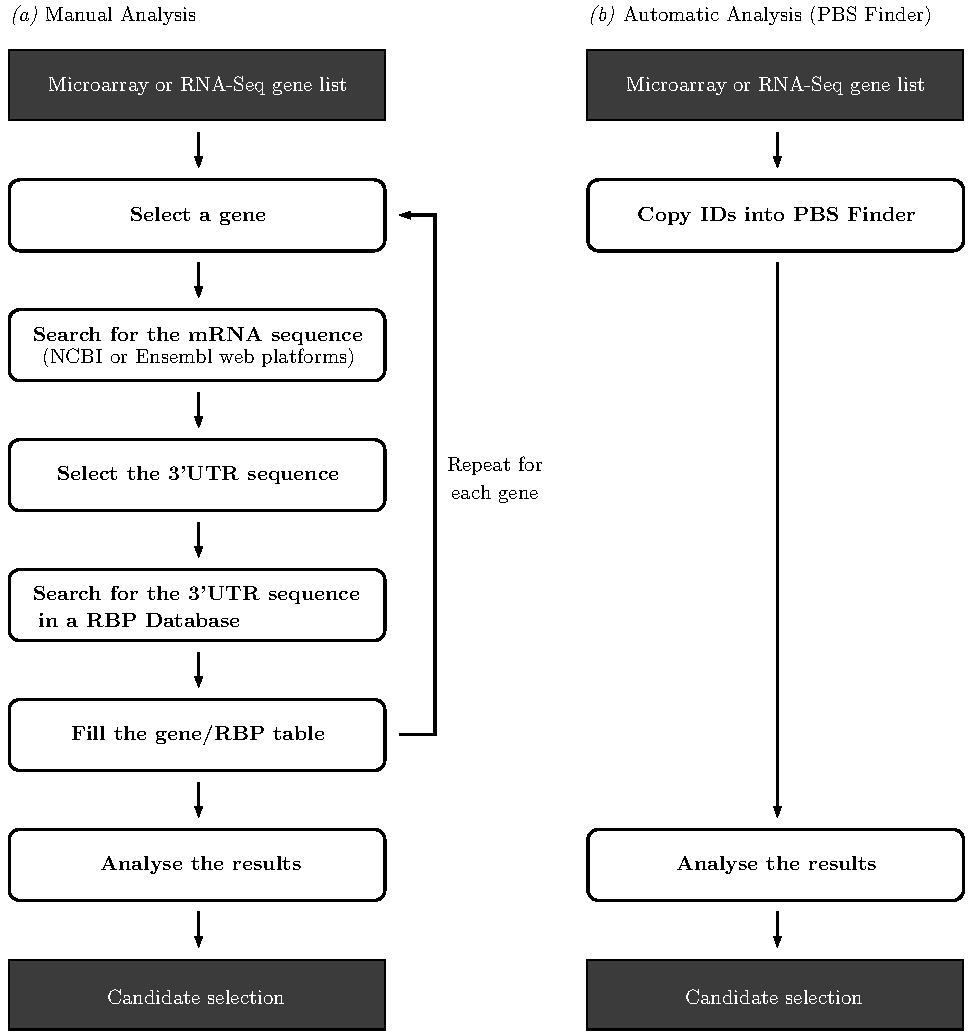
\includegraphics[width=\textwidth]{oldvsnew}
    \caption[Comparison between manual RBP analysis and automatic RBP analysis (conducted with PBS Finder)]{
      Comparison between manual RBP analysis and automatic RBP analysis
      (conducted with PBS Finder).
    }
    \label{fig:oldvsnew}
  \end{center}
\end{figure}

The first step is to select a gene for analysis. The gene identifier is then
searched in either Ensembl or NCBI web platforms, depending on the type of the
identifier. If the gene is found in those platforms, the next step involves
finding the 3'UTR sequence in the results page and copying it. That sequence is
then passed to an online RBP analysis platform, that should retrieve a list of
RBPs that may bind to that particular sequence. Lastly, the RBP information must
be manually combined in the results table. When this information is collected
for every gene it is finally possible to conduct a useful analysis.

On the other hand, with PBS Finder the user needs only to provide the complete
list of all gene identifiers in the data set. The tool will them automatically
process those identifiers, find all relevant information and present it to the
user, ready for further analysis. Note that these results contain additional
information that is not available in the manual analysis: gene, transcript and
protein information (names, additional sequences, pathways, etc.); links to
external platforms; useful histograms; and gene and protein clustering results.

\subsection{Efficiency}

It is essential that the developed platform is able to conduct the analysis in a
timely fashion, making tool performance a major concern. As such, we compared
the average time that an expert would take to analyse the data set to the
average time that the tool takes to analyse the same data set.

The consulted molecular biology expert estimated that, on average, it would take
thirty minutes to analyse a single gene. This means that an expert would need an
average of eleven and a half hours ($30\ minutes \times 23\ genes$) to process the
entire case study data set.

On the other hand, the automated tool takes a shorter amount of time to conduct
the analysis of the same data set. In order to assess the actual amount of time
the tool took to analyse the entire data set we ran twenty sequential
experiences, ten for each of the experimental environments. Table \ref{tab:perf}
depicts the duration of each one of those experiments, as well as their average
duration. As expected, an automated tools widely outperforms a human expert in
information collection and analysis.

\begin{table}[!htb]
  \centering
  \begin{tabular}{{l} | {l}{l}}
    & \textbf{\emph{machine1}} & \textbf{\emph{machine2}}\\ \hline
    \textbf{\emph{Experience 1}}    & $1m\ 47s$ & $6m\ 34s$\\
    \textbf{\emph{Experience 2}}    & $1m\ 58s$ & $6m\ 25s$\\
    \textbf{\emph{Experience 3}}    & $1m\ 46s$ & $6m\ 30s$\\
    \textbf{\emph{Experience 4}}    & $1m\ 45s$ & $6m\ 15s$\\
    \textbf{\emph{Experience 5}}    & $2m\ 23s$ & $6m\ 42s$\\
    \textbf{\emph{Experience 6}}    & $1m\ 35s$ & $6m\ 30s$\\
    \textbf{\emph{Experience 7}}    & $1m\ 40s$ & $6m\ 31s$\\
    \textbf{\emph{Experience 8}}    & $1m\ 39s$ & $6m\ 11s$\\
    \textbf{\emph{Experience 9}}    & $1m\ 42s$ & $6m\ 42s$\\
    \textbf{\emph{Experience 10}}   & $1m\ 42s$ & $6m\ 52s$\\ \hline
    \textbf{\emph{Average time}}    & $1m\ 42s$ & $6m\ 31s$\\
  \end{tabular}

  \caption[Execution times of the case study data set in two different environments]{
    Execution times of the case study data set in two different environments
    (sequential experiments). Note that while \emph{machine2} has a significant
    loss in performance (due to its outdated hardware) it still achieves
    satisfactory execution times. This test also shows that it is possible to
    efficiently run PBS Finder in a home computer.
  }
  \label{tab:perf}
\end{table}

\section{Chapter Conclusions}

Through this case study we have shown that PBS Finder produces relevant and
correct results for large-scale analysis of RBPs using data from \ngs{}
techniques. We have also shown that our tool significantly facilitates the work
of the biologist, by making analysis of this data easier and quicker. As such,
we consider PBS Finder a tool of great value for studying RNA biology.

